\documentclass{beamer}
\usepackage[utf8]{inputenc}
\usepackage{graphics}
\mode<presentation> {
\usetheme{unc}}
\setbeamertemplate{navigation symbols}{} % To remove the navigation symbols from the bottom of all slides uncomment this line

\usepackage{graphicx} % Allows including images
\usepackage{booktabs} % Allows the use of \toprule, \midrule and \bottomrule in tables


\usepackage{hyperref}
\hypersetup{linkcolor=blue,colorlinks=true}


% Remove symbols
\beamertemplatenavigationsymbolsempty


%\usetheme{default}

\usefonttheme{serif}

%----------------------------------------------------------------------------------------
%	TITLE PAGE
%----------------------------------------------------------------------------------------


\title[IPE Core Concepts]{\LARGE{Core Concepts of Intl. Political Economy (IPE) and Intl. Governance of Trade}}
\author[POLI 150]{Steven Saroka}
\institute{POLI 150}
\date{19 March 2024}


\begin{document}

\begin{frame}
\titlepage % Print the title page as the first slide
\end{frame}


%\begin{frame}
%\frametitle{Overview} % Table of contents slide, comment this block out to remove it
%\tableofcontents % Throughout your presentation, if you choose to use \section{} and \subsection{} commands, these will automatically be printed on this slide as an overview of your presentation
%\end{frame}


%%% SLIDE TEMPLATES

% Template for images
% \begin{frame}{\LARGE Kurdistan}
%     \centering
% \includegraphics[width=\textwidth,height=0.8\textheight,keepaspectratio]{}
% \end{frame}

% %% Core template for the slides
% \begin{frame} 
% \frametitle{\LARGE{}}
% \end{frame}

%----------------------------------------------------------------------------------------
%	PRESENTATION SLIDES
%----------------------------------------------------------------------------------------



\begin{frame} 
	\frametitle{\LARGE{Today's Class}}
	\begin{itemize}
		\Large{

			\item Foundational concepts of IPE
		}
	\end{itemize}
\end{frame}


\begin{frame} 
	\frametitle{\LARGE{Key Terms}}
	\begin{itemize}
		\item Globalization
		\item Comparative Advantage
		\item Absolute Advantage
		\item Heckscher-Ohlin Trade Theory
		\item Protectionism
		\item Tariffs
		\item WTO
	\end{itemize}
\end{frame}


\begin{frame} 
	\frametitle{\LARGE{Central Question}}
    \centering
		\Large{How does the economy matter for international relations?}
\end{frame}

\begin{frame} 
	\frametitle{\LARGE{Shift to IPE}}
	\begin{itemize}
		\item This second half of the class will shift focus away from political violence to discuss economic topics. \pause
		\item \textbf{International Political Economy}: the study of how and when international economic integration occurs, and how this impacts domestic politics. \pause
		\item Understanding the ``political" in IPE means understanding the ``economy" first! \pause 
		\item If any concepts are unclear, please ask questions!  
	\end{itemize}
\end{frame}

\begin{frame} 
	\frametitle{\LARGE{Globalization Definition}}
IPE is fundamentally linked to the process of globalization.
	\begin{itemize}
			\item \textbf{Globalization}: international economic integration. \pause
			\item This describes the  increasing integration of national economies into international networks, as economic exchange spreads across borders. These components include: \pause
			\begin{itemize}
				\item Goods and services
				\item Intellectual property
				\item Money (``capital")
				\item People \pause
			\end{itemize}
		\item As a result, the economy of almost every state is now linked to a broader, global economic system.
	\end{itemize}
\end{frame}

\begin{frame} 
	\frametitle{\LARGE{Globalization}}
The process of globalization has several implications:
	\begin{itemize}
		\item \textbf{Consequences for government sovereignty:} state economies are now influenced by actors other than the state. \pause 
		\item \textbf{Opportunities for growth:} states may be able to sell their goods and services to new buyers, potentially growing their economies. \pause
		 \item \textbf{Potential for crisis:} economic crashes rarely stay contained within a single state. \pause 
		\item Domestic and international politics \textbf{both} matter for economic policy. \pause 
		\item Globalization generates common and conflicting interests both within and across states.	
	\end{itemize}
\end{frame}

\begin{frame} 
	\frametitle{\LARGE{Eras of Economic Globalization}}
	\begin{itemize}
			\item \textbf{British Gold standard:} the decades before WWI, and afterwards up to the 1929 economic crash. \pause 
			\\~\\ 
			\item \textbf{Bretton Woods/US Gold Standard:} WWII until 1971. \pause 
			\\~\\
			\item \textbf{(Hyper)globalization:} approximately 1970s until present. \pause
			\\~\\
			\item \textbf{Backlash}: 2010 to present?
		\end{itemize}
\end{frame}

\begin{frame} 
	\frametitle{\LARGE{Globalization over Time}}
	\begin{itemize}
	\item The spread of globalization can be measured empirically. The following slides show indicators from the \href{https://kof.ethz.ch/en/forecasts-and-indicators/indicators/kof-globalisation-index.html}{KOF Swiss Economic Institute}. \pause
	\item These measure globalization both \textit{de facto} and \textit{de jure}: both real indicators of globalization as well as legal and regulatory indicators of it.
	\end{itemize}
\end{frame}

\begin{frame} 
	\frametitle{\LARGE{Dimensions of Globalization}}
	\begin{itemize}
		\item Social: cross-border contacts of all kinds. \pause
		 \begin{itemize}
		 	\item De facto: international tourism, students, migration, information flows, cultural goods, etc.
		 	\item De jure: telecommunications access, press freedom, spread of civil liberties and human rights, freedom to travel. \pause
		 \end{itemize}
		\item Political: international institutions. \pause 
			\begin{itemize}
				\item De facto: Embassies, UN peacekeeping, international NGOs.
				\item De jure: international organizations and treaties, as well as diversity of states in them. \pause
			\end{itemize}
		\item Economic: economic exchanges. \pause
		\begin{itemize}
			\item De facto: trade in goods and services, FDI and capital flows, etc.
			\item De jure: trade regulations, taxes, tariffs, investment and capital restrictions. 
		\end{itemize}
	\end{itemize}
\end{frame}

\begin{frame}{\LARGE Social Globalization}
    \centering
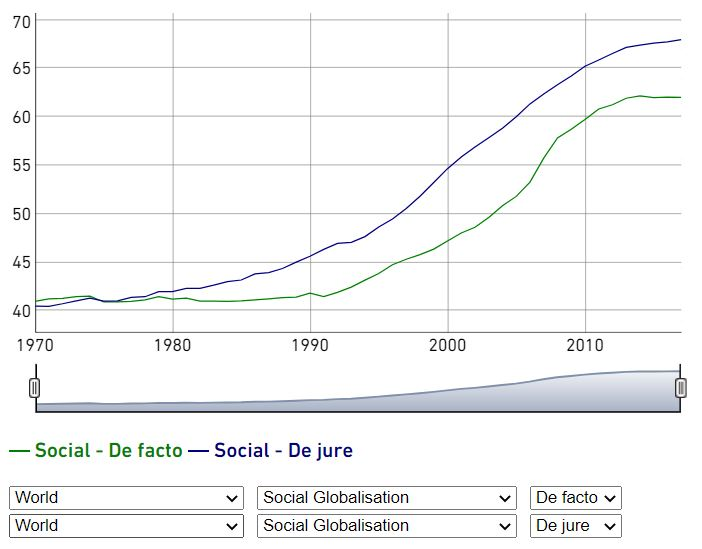
\includegraphics[width=\textwidth,height=0.8\textheight,keepaspectratio]{KOF social.JPG}
\end{frame}


\begin{frame}{\LARGE Political Globalization}
    \centering
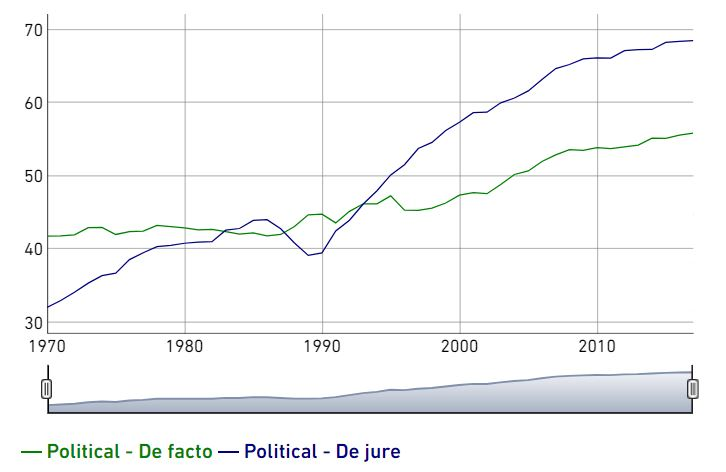
\includegraphics[width=\textwidth,height=0.8\textheight,keepaspectratio]{KOF political.JPG}
\end{frame}


\begin{frame}{\LARGE Economic Globalization}
    \centering
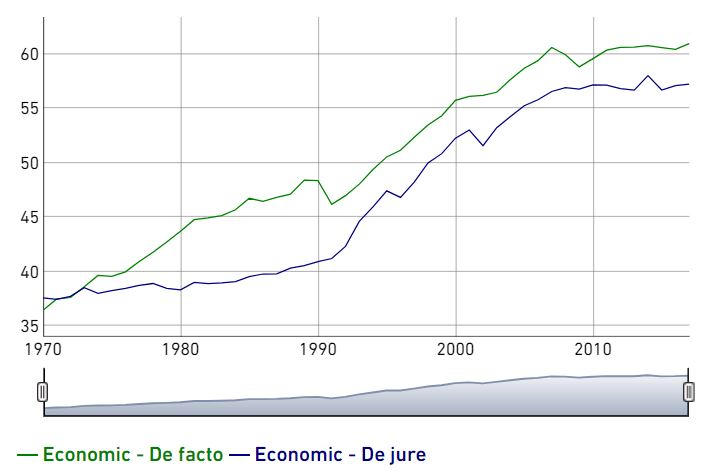
\includegraphics[width=\textwidth,height=0.8\textheight,keepaspectratio]{KOF economic.JPG}
\end{frame}


\begin{frame} 
\frametitle{\LARGE{Comparative and Absolute Advantage}}
\begin{itemize}
    \item So, what determines what products and services firms and states send out into this global economy? 
    \item Answering this means first defining \textbf{comparative advantage} and \textbf{absolute advantage}.
    \item Extended example: mowing one's lawn.
\end{itemize}
\end{frame}

\begin{frame} 
	\frametitle{\LARGE{Comparative and Absolute Advantage}}
	\begin{itemize}
		\item Imagine a UNC alum and her neighbor, a Duke alum, both of whom live in identical houses with identical-sized lawns. \pause
		\item Suppose the UNC alum in question is both brilliant and a fabulous athlete.  \pause
		\item This UNC alum can mow her lawn faster than anyone else, \textbf{but should she?}  
	\end{itemize}
\end{frame}

\begin{frame} 
	\frametitle{\LARGE{Comparative and Absolute Advantage}}
	\begin{itemize}
		\item The UNC alum can mow her lawn in 2 hours. \pause
		\item The Duke alum could mow the UNC alum’s lawn in 4 hours. \pause
		\item The UNC alum thus has an \textbf{absolute advantage} in mowing lawns. \pause
		\item \textbf{Absolute advantage}: the ability of a producer to generate a greater number of goods than other producers using the same starting amount of resources.
	\end{itemize}
\end{frame}

\begin{frame} 
	\frametitle{\LARGE{Comparative and Absolute Advantage}}
	\begin{itemize}
		\item Suppose that those same 2 hours, the UNC alum's next best alternative work would be to make \$1000 as a consultant. \pause
		\begin{itemize}
			\item Thus, UNC alum's \textbf{opportunity cost} for mowing the lawn is \$1000. \pause 
		\end{itemize}
		\item Suppose also that the Duke alum’s next best alternative to mowing a lawn is serving drinks at a local bar for \$8 per hour.  \pause
		\begin{itemize}
			\item Thus, Duke alum's \textbf{opportunity cost} for mowing the lawn is \$32, as it would take them 4 hours to mow the lawn.
		\end{itemize}
	\end{itemize}
\end{frame}

\begin{frame} 
	\frametitle{\LARGE{Comparative and Absolute Advantage}}
	\begin{itemize}
		\item Our UNC alum has an absolute advantage in mowing lawns because they can do the same amount of work in less time.		
		\item But our Duke alum has a \textbf{comparative advantage} in mowing lawns because he has the lower opportunity cost (\$32 $<$ \$1000). \pause
		\item \textbf{Comparative advantage}: the ability of a producer to generate a good more efficiently than other goods it could create, so that its most efficient use of resources is to make that specific good/service. \pause 
		\item Another way to say this is that an actor has a comparative advantage if they can produce a good/service at a lower opportunity cost than other actors.
	\end{itemize}
\end{frame}

\begin{frame} 
	\frametitle{\LARGE{Comparative and Absolute Advantage}}
	\begin{itemize}
		\item What does this imply?
		\item Rather than mowing her lawn, our UNC alum should work as a consultant and hire our Duke alum to mow the lawn. \pause
		\item As long as the UNC alum pays the Duke alum more than \$32 and less than \$1,000, \textbf{both of them are better off than they would be otherwise.} \pause
		\item \textbf{All actors have a comparative advantage in producing something, even if they have an absolute advantage in nothing.} \pause
		\item Now, scale this up to the level of international economics...		
	\end{itemize}
\end{frame}

\begin{frame} 
	\frametitle{\LARGE{Comparative and Absolute Advantage}}
	\begin{itemize}
		\item States also have comparative advantages in producing goods and services.
		\item Economics, going all the way back to Adam Smith's \textit{Wealth of Nations} (1776), has recognized the benefits of specializing production. \pause
		\item Assuming prerequisites are met (including a large enough market to sell all those goods that are produced by specialized producers, and a free market), \textbf{production according to comparative advantage will result in more goods being available at the cheapest possible price}. 
	\end{itemize}
\end{frame}

\begin{frame} 
	\frametitle{\LARGE{Comparative and Absolute Advantage}}
	\begin{itemize}
		\item \textbf{This implies that free trade, where all producers can specialize by producing the goods for which they have a comparative advantage, can be mutually beneficial. This still holds even if one state has an absolute advantage in producing all goods.}
	\end{itemize}
\end{frame}

\begin{frame} 
	\frametitle{\LARGE{Free Trade vs. Mercantilism}}
	\begin{itemize}
		\item Smith, and other economists of his era like David Ricardo (1772-1823), thus clashed with the \textbf{mercantilist} thinking of their era. \pause
		\item Recall that mercantilism explicitly prevented free trade, restricting trade within an empire via \textbf{trade barriers}: state restrictions on the international flow of goods and services. \pause
		\item Eventually, free trade and globalization won out, leading to the eras of globalization from prior slides.
	\end{itemize}
\end{frame}

\begin{frame} 
	\frametitle{\LARGE{Grand Theories of IPE}}
This theoretical struggle is also captured by the grand theories of IPE:
	\begin{itemize}
			\item \textbf{Liberalism:} government should be separated from markets (also sometimes referred to as free trade or capitalism.) \pause 
			\item \textbf{Mercantilism:} governments direct and restrict the economy (also sometimes called economic nationalism). \pause 
			\item \textbf{Marxism:} the structure of economy determines politics, necessitating the importance of collective ownership of the means of production by workers.  
	\end{itemize}
\end{frame}

\begin{frame}{\LARGE Grand Theories}
    \centering
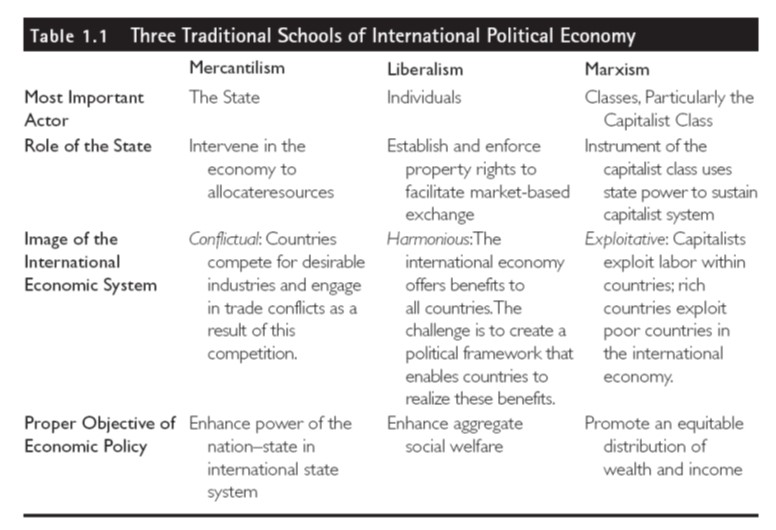
\includegraphics[width=\textwidth,height=0.8\textheight,keepaspectratio]{grand theories.jpg}
\end{frame}

\begin{frame} 
	\frametitle{\LARGE{Heckscher-Ohlin Trade Theory}}
	\begin{itemize}
		\item States (their industries) tend to have a comparative advantage in producing \textit{something}, but how do we determine what that thing is? 
		\item \textbf{Heckscher-Ohlin trade theory} is one attempt to answer this, and was highly influential on following economic theory.
		\item This theory starts by classifying a state's \textbf{factors of production}: \pause
		\begin{enumerate}
			\item Land: farming or natural resource extraction. \pause
			\item Labor: generally unskilled labor. \pause
			\item Capital: financial capital and equipment. \pause
			\item Human capital: skilled labor (sometimes combined with Capital).
		\end{enumerate}
	\end{itemize}
\end{frame}

\begin{frame} 
	\frametitle{\LARGE{Heckscher-Ohlin Trade Theory}}
	\begin{itemize}
		\item HO trade theory predicts that the relative amounts of these factors within a state determine its comparative advantage in production. \pause
		\item \textbf{States with an abundance of a given factor will have a comparative advantage in producing goods that use that factor, and so will export goods based on that factor.} The inverse is also true: \pause
		\item States will import goods that require factors which are scarce in the state, as they will not have a comparative advantage in producing them. 
	\end{itemize}
\end{frame}

\begin{frame}{\LARGE Heckscher-Ohlin Trade Theory}
	\centering
	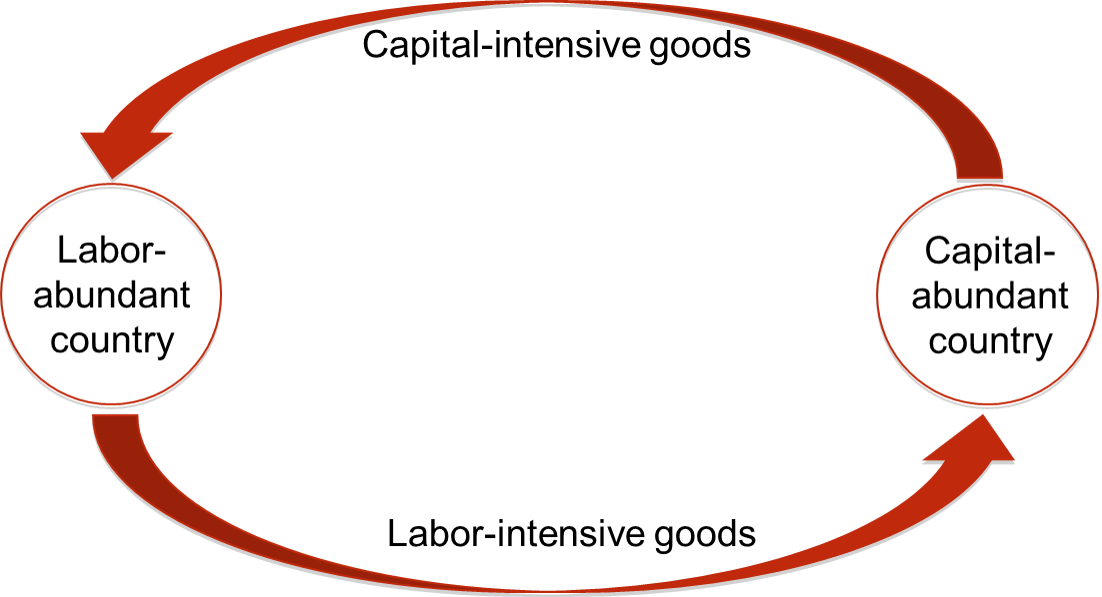
\includegraphics[width=\textwidth,height=0.8\textheight,keepaspectratio]{HOillustration.png}
\end{frame}

\begin{frame} 
	\frametitle{\LARGE{HO and Competing Theories}}
	\begin{itemize}
		\item Heckscher-Ohlin is not the only theory of comparative advantage for a state's economy, but it influenced subsequent theories (like Ricardo-Viner trade theory). \pause
		\item Equally importantly, it establishes a way to broadly classify elements of the state's economy. \pause
		\item This topic will come up in the next lecture.
	\end{itemize}
\end{frame}

\begin{frame} 
	\frametitle{\LARGE{Trade Barriers and Protectionism}}
	\begin{itemize}
		\item Despite the economic consensus that production according to comparative advantage in a system of free trade will maximize available goods and minimize prices, states routinely create \textbf{trade barriers}: government limits on the international exchange of goods. \pause
		\item Usually these barriers are synonymous with \textbf{protectionism}: state-imposed barriers to imports.
	\end{itemize}
\end{frame}

\begin{frame} 
	\frametitle{\LARGE{Methods of Protectionism}}
Protectionism can take several forms:
	\begin{itemize}
		\item \textbf{Tariff}: tax on an import, raising the domestic price of that imported good. Tariffs are paid by the importer. \pause
		\item \textbf{Quota}: restriction on how much of a foreign good can be imported. \pause
		\item \textbf{Nontariff barriers}: rules often related to quality of imports that naturally restrict quantity. 
	\end{itemize}
Practically every state in the international system engages in protectionism, most commonly via tariffs, but tariff rates have fallen over time. 
\end{frame}

\begin{frame}{\LARGE Tariff Rates Over Time}
	\centering
	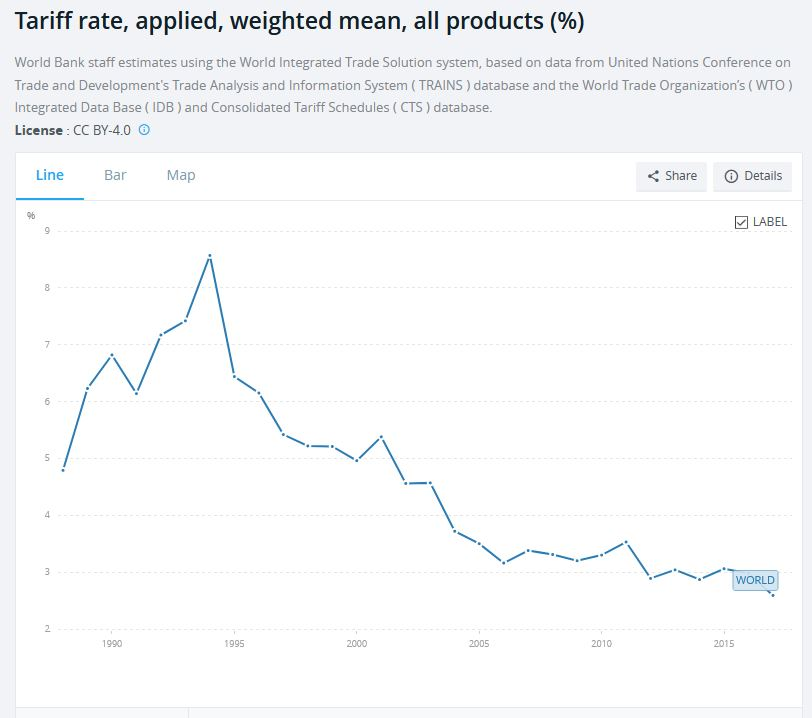
\includegraphics[width=\textwidth,height=0.8\textheight,keepaspectratio]{tariff rate over time.JPG}
\end{frame}

\begin{frame} 
	\frametitle{\LARGE{International Institutions and Trade}}
This decline in tariffs, and accompanying increase in free trade, has its roots in post-WWII rebuilding.
	\begin{itemize}
		\item In the postwar era, Western leaders tried to create institutions to prevent future conflict. \pause
		\item While the UN was part of this, they were also motivated by the belief that economic integration would make war recurrence less likely. \pause
		\item This led to the creation of the Bretton Woods institutions, of which the relevant one for trade is the World Trade Organization (originally called the GATT when it was formed in 1947, with formal change to WTO in 1995). \pause
				\item \textbf{The WTO's goal is to encourage multilateral reduction of trade barriers, and also provide a dispute resolution mechanism.}
	\end{itemize}
\end{frame}

\begin{frame} 
	\frametitle{\LARGE{International Institutions and Trade}}
	\begin{itemize}
		\item Why is the WTO necessary in the first place? \pause
		\item The choice between free trade and protectionism is effectively a Prisoner's Dilemma...
	\end{itemize}
\end{frame}

\begin{frame}{\LARGE Tariffs and Free Trade}
	\centering
	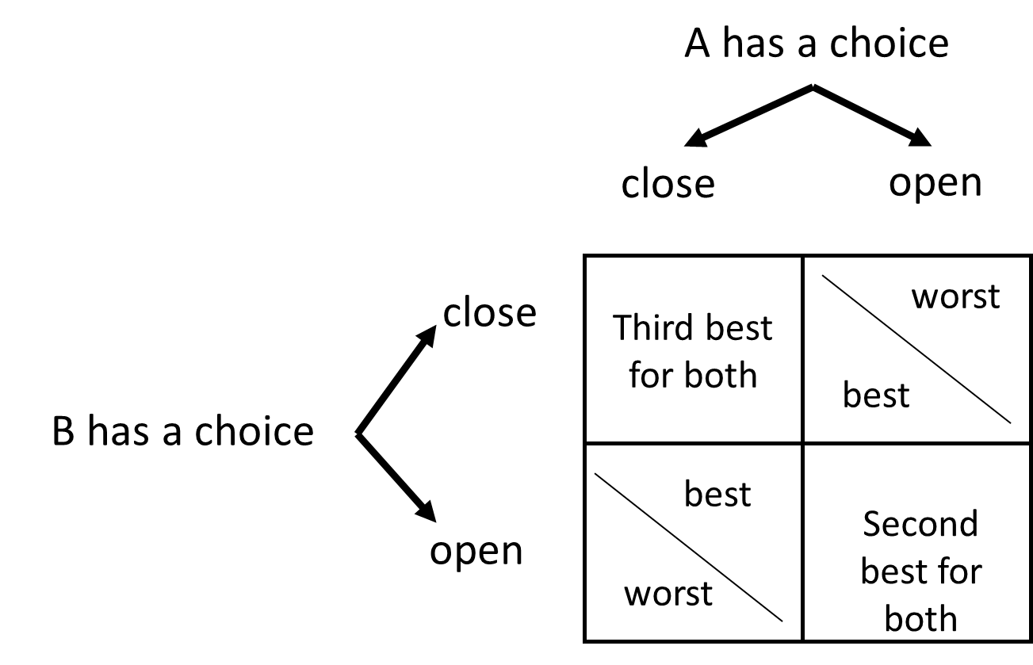
\includegraphics[width=\textwidth,height=0.8\textheight,keepaspectratio]{freetradePD.png}
\end{frame}

\begin{frame} 
	\frametitle{\LARGE{Trade as Prisoner's Dilemma}}
	\begin{itemize}
			\item Best outcome: you don't lower your trade barriers (close) and the other country lowers theirs (open). \pause 
			\item Second-best outcome: both countries lower/remove trade barriers (known as trade liberalization). \pause
			\item Worst outcome: you lower your trade barriers and the other country does not. \pause
			\item The incentive structure of the situation gives both countries an incentive to defect by engaging in protectionism. 
	\end{itemize}
\end{frame}

\begin{frame} 
	\frametitle{\LARGE{WTO Solutions}}
	\begin{itemize}
		\item The WTO helps to foster cooperation by creating rules for members. \pause
		\item The most important is \textbf{Most Favored Nation} status: all members of the WTO must treat all other members the same as their most favored trading partners (that is, those partners with whom they have the fewest trade barriers). \pause
		\item WTO also provides a way to resolve trade disputes via the \textbf{Dispute Settlement Body}. \pause
		\item If a state is found to be in violation of WTO rules, the WTO permits the other state to impose trade protection of equal value. \pause
		\item WTO rules are “self-enforcing” – they work by letting states punish other states ``legally.”
	\end{itemize}
\end{frame}

\begin{frame} 
	\frametitle{\LARGE{WTO Over Time}}
	\begin{itemize}
			\item The GATT/WTO has evolved and expanded since WWII over several rounds of negotiations, which have generally involved reducing remaining barriers to free trade. \pause
			\item Negotiations stalled after the start of the Doha Round (2001), and by 2015 it was clear that the WTO had lost organizational momentum.
			\item This led to the rise of...
	\end{itemize}
\end{frame}

\begin{frame} 
	\frametitle{\LARGE{Preferential Trade Agreements}}
	\begin{itemize}
			\item \textbf{Preferential trade agreements} (PTAs) (also called Regional Trade Agreements) have proliferated since the WTO has stalled. \pause
			\item These can be regional (ex: NAFTA) or bilateral, but are never global like the WTO is. \pause
			\item They serve the same monitoring and dispute resolution functions, but are easier to negotiate due to fewer members. \pause
			\item Have grown increasingly complex (including ties to human rights).
	\end{itemize}
\end{frame}

\begin{frame}{\LARGE PTAs Worldwide}
	\centering
	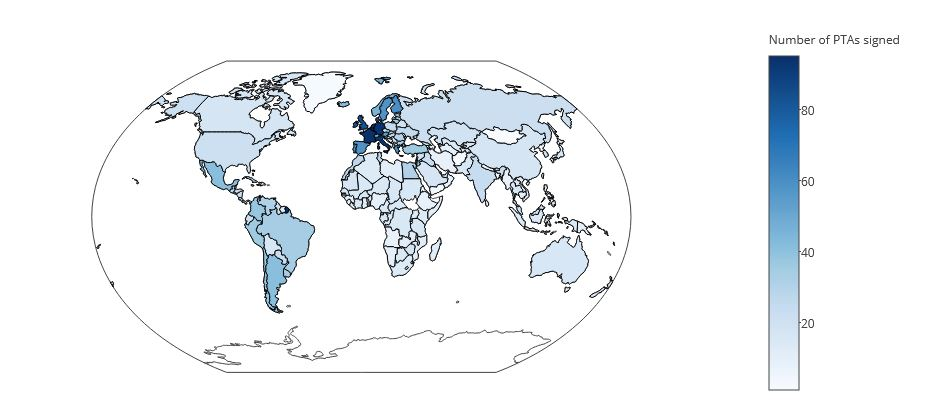
\includegraphics[width=\textwidth,height=0.8\textheight,keepaspectratio]{number of PTAs.JPG}
\end{frame}

\begin{frame}{\LARGE Selected PTAs Worldwide}
	\centering
	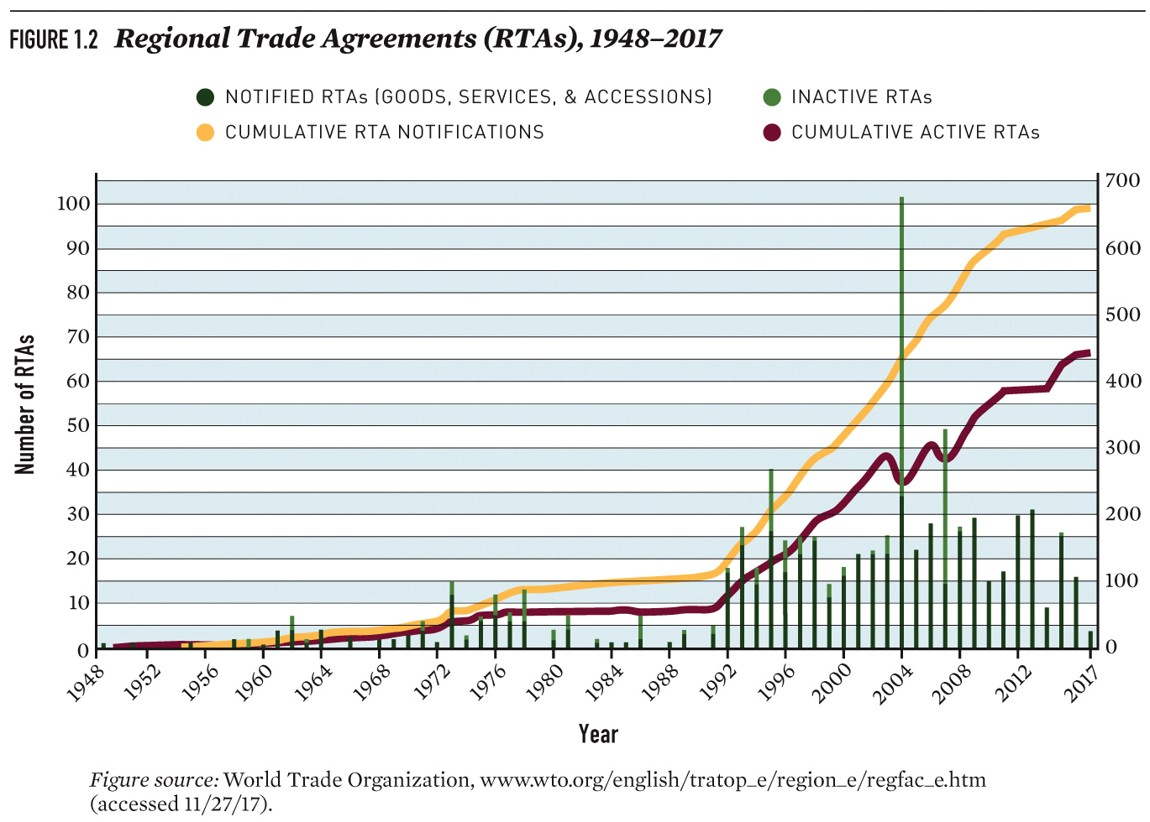
\includegraphics[width=\textwidth,height=0.8\textheight,keepaspectratio]{RTAs.JPG}
\end{frame}

\begin{frame} 
	\frametitle{\LARGE{WTO Shortcomings}}
	\begin{itemize}
		\item WTO has been criticized as especially responsive to rich developed states (most of whom used protectionism while becoming rich and developed) and neglecting the interests of poorer states. \pause
		\item Many poorer states with primarily agricultural economies view the WTO as stacked against their interests for insisting on lowering trade barriers while allowing rich states like the US to keep agricultural subsidies in place. \pause
		\item WTO has also been criticized for prioritizing economic liberalization over environmental protection.
	\end{itemize}
\end{frame}

\begin{frame} 
	\frametitle{\LARGE{Closing Questions}}
	\centering
	\Large{Do the benefits of free trade accrue equally to all citizens? Does this have any relation to the persistence of protectionism?} 
\end{frame}

\end{document}
